\documentclass{article}
\input{artisynthDoc}
\usepackage{enumitem}

\iflatexml
\else
% reset fancyhr settings set by artisynthDoc
\fancyhead[L,C,R]{}
\fancyfoot[L,R]{}
\fancyfoot[C]{\thepage}
\renewcommand{\headrulewidth}{0pt}
\renewcommand{\footrulewidth}{0pt}
\fi

\def\ArtHome[#1]{{\tt <ARTISYNTH\_HOME>#1}}

\title{ArtiSynth Quick Installation Guide}
\author{John Lloyd}
\setpubdate{Last updated: October, 2026}
\iflatexml
\date{}
\fi

\newif\ifNeedLibraryPath
\NeedLibraryPathfalse

\begin{document}

%\maketitle

\iflatexml{\large\pubdate}\fi

%\tableofcontents

% add title in PDF version
\iflatexml\else
\begin{center}
{\sffamily\Large\bfseries ArtiSynth Quick Installation Guide}
\end{center}
\bigskip
\fi

This describes how to quickly install one of the precompiled versions of
ArtiSynth, which can be useful for users wanting to test the system and run the
demonstration programs. Once you decide to use ArtiSynth to build models, we
instead recommend installing the latest version from Github into the Eclipse
IDE, as described here for
\artisynthManual[installation/windowsInstallation]{windowsGitEclipseInstall}{Windows},
\artisynthManual[installation/macosInstallation]{macosGitEclipseInstall}{MacOS},
and
\artisynthManual[installation/linuxInstallation]{linuxGitEclipseInstall}{Linux}.

\section{Instructions}

\subsection{To install ArtiSynth:}

\begin{enumerate}

\item You need a 64 bit Windows, MacOS, or Linux system based on an Intel
processor. MacOS systems based on the new Apple ARM processor (the M
chips) implement a compatibility layer (called Rosetta) that should allow
ArtiSynth to run as is, provided that you use a 64-bit {\it Intel-based} Java
development kit (JDK).

\item A 64-bit Java development kit (JDK) should be installed. This should be
an Intel-based JDK (containing {\tt x64} in its download name); on ARM-based
MacOS machines, this should run using the Intel compatibility layer.
You will need a full Java Development Kit (JDK), not simply a runtime
environment (JRE), and it should have version 21 or higher (Java 21 is
recommended if you plan to use ArtiSynth with MATLAB). If you need
a JDK, we suggest Eclipse Temurin, available from
\href{https://adoptium.net/temurin/releases/}%
{adoptium.net/temurin/releases}.
 
\item To verify that the Java JDK is visible to your system, open a
terminal window (e.g., {\tt CMD} on Windows), run the command {\tt
javac -version}, and check that the version matches the JDK.  If it
does not, follow the instructions in Section
\ref{MakingJDKVisible}.

\item Download the latest precompiled ArtiSynth release 
(e.g., {\tt artisynth\_core\_3.8.zip}) from
\iflatexml\else\\\fi % need a newline in PDF version
\href{https://www.artisynth.org/downloads}{www.artisynth.org/downloads}.
 
\item Unzip the file into a folder, preferably one without spaces in the
name.

\end{enumerate}
 
\subsection{To run ArtiSynth:}

\begin{itemize}[leftmargin=26pt]
 
\item On Windows: click {\tt bin\BKS artisynth.bat} under the install folder. 
 
\item On MacOS or Linux: use a terminal to run {\tt bin/artisynth} 
under the install folder.

\item[\ ] To run demos, open the {\tt Models} menu at the top and
choose the model you would like. It will be loaded and displayed in
the viewer. To start/stop simulation, use the play button

\includegraphics[width=0.15in]{images/playButton} at the top right.

\begin{sideblock}
On MacOS, running a model may initially produce a security error because of
untrusted ArtiSynth native libraries.  See Section \ref{MacOSSecurity} for
details on handling this.
\end{sideblock}

\end{itemize}

\subsection{To make changes to a demo:}

\begin{enumerate}

\item If {\tt <AT>} denotes the top-level folder of your ArtiSynth
installation, then add {\tt <AT>\BKS bin} (Windows) or {\tt <AT>/bin} (MacOS
and Linux) to your system Path as described in Section \ref{SettingPath}.

\item Edit the {\tt .java} file for the demo, which will be located
in a folder under {\tt <AT>\BKS src\BKS artisynth\BKS demos},
using a plain text editor (e.g., {\tt notepad} on Windows).

\item From within a terminal window (e.g., {\tt CMD} on Windows), go to the
demo folder and enter the command {\tt compile}.

\end{enumerate}

\section{Making the JDK visible to your system}
\label{MakingJDKVisible}

It is important to ensure that the JDK is visible to your system and
supersedes any other Java installations.

\subsection{Windows and Linux}

If {\tt <JDK>} denotes the top-level folder of your installed JDK,
then add the folder {\tt <JDK>\BKS bin} (Windows) or {\tt <JDK>/bin}
(Linux) to your system Path, using the instructions given in Section
\ref{SettingPath}. The folder should be added {\it ahead} of any other
Java installations that might be specified on the Path.

On Windows, {\tt <JDK>} is usually something like
\begin{verbatim}
   C:\Program Files\Eclipse Adoptium\jdk-21.0.8.9-hotspot
\end{verbatim}
for Temurin, or 
\begin{verbatim}
   C:\Program Files\Java\jdk-21
\end{verbatim}
for Oracle. The Windows JDK installer usually makes the JDK visible
automatically.

\subsection{MacOS}

On MacOS, you can set the ``default'' JDK by setting the {\tt JAVA\_HOME}
environment variable.  This can be done inside the initialization file for your
command line shell.  Assume that the desired JDK has version number {\tt 21}
and that your home directory is {\tt <HOMEDIR>}.

\begin{itemize}

\item If your command line shell is {\tt zsh} (which it will be by
default), then the initialization file is {\tt <HOMEDIR>/.zshrc}. Use a
plain text editor to edit (or create) this file and insert a line of
the form
%
\begin{lstlisting}[]
  export JAVA_HOME=`/usr/libexec/java_home -v 21`
\end{lstlisting}
%
The same line can be used if your shell is {\tt bash}, in which case
the initialization file is {\tt <HOMEDIR>/.bashrc}.

\item If you have changed your shell to {\tt csh} or {\tt tcsh},
then the initialization file is {\tt <HOMEDIR>/.cshrc}. Use a plain text editor
to edit or create this file and insert a line of the form
%
\begin{lstlisting}[]
  setenv JAVA_HOME `/usr/libexec/java_home -v 21`
\end{lstlisting}
%

\end{itemize}

Note that in both examples above, the left quote character "{\tt \`{}}" is used
instead of the more common right quote "{\tt '}".

Setting {\tt JAVA\_HOME} can also be done directly within the shell;
doing it within the initialization file simply avoids the need to do
so each time a new terminal window is opened.

\section{Adding Directories to the System Path}
\label{SettingPath}

The system ``Path'' is a list of directories which the system searches
in order to find executables. Adding a directory to the path allows
executables contained in that directory to be called directly from a
command window (such as {\tt CMD} on Windows).

\subsection{Windows}

\begin{enumerate}

\item Open the {\sf Start} search, enter ``{\tt env}'', and choose
{\sf ``Edit the system environment variables''}.

\item Click on {\sf Environment Variables}.

\item Under {\sf User variables} (the top window), click on {\sf Path}
and click {\sf Edit}. If {\sf Path} does not exist, click {\sf New}.

\item In the {\sf Edit environment variable} dialog, click {\sf New}
and enter the full path name for each directory you wish to add.

\item Close {\it all} dialogs by clicking {\sf OK} and restart 
your command window.

\end{enumerate}

For example, if ArtiSynth is installed at {\tt C:\BKS artisynth\BKS
artisynth\_core}, then you would add the directory
\begin{verbatim}
  C:\artisynth\artisynth_core\bin
\end{verbatim}

\subsection{MacOS}

Since MacOS is a Unix-based system, directories can be added to the
path by editing the {\tt PATH} environment variable directly in the
initialization files for whichever command line shell you are using,
in the same manner as described for Linux (Section \ref{Linux}).
The default command line shell for MacOS is {\tt zsh}.

On MacOS, directories can also be added to the
path by adding a text file containing the directories to {\tt
/etc/paths.d}.  In particular, we can create a file called {\tt
ArtiSynth} in {\tt /etc/paths.d} that contains the full path names of
the desired directories.

\begin{enumerate}

\item Open a terminal window

\item Use {\tt sudo} to create {\tt /etc/paths.d/ArtiSynth} with a plain
text editor. For example:
\begin{verbatim}
  sudo nano /etc/paths.d/ArtiSynth
\end{verbatim}

\item Add the full path name of each desired directory, one per line,
and save the file.

\item To test the revised {\tt PATH}, open a new terminal
window and enter the command: {\tt echo \$PATH}.

\end{enumerate}

\subsection{Linux}
\label{Linux}

On Linux, directories can be added to the path by appending them to
the {\tt PATH} environment variable, which is a list of directories
separated by colons `{\tt :}'. The most direct way to do this is to
redefine {\tt PATH} inside one of the initialization files for
whichever command line shell you are using.

Assume that your home folder is {\tt <HOMEDIR>}. Then for the {\tt
zsh} shell (the default on MacOS), one can edit {\tt
<HOMEDIR>/.zshrc}, or for the {\tt bash} shell (the usual default on
Linux), {\tt <HOMEDIR>/.bashrc} (creating the file if it does not
already exist), and insert a line of the form
\begin{verbatim}
   export PATH=<DIR>:$PATH
\end{verbatim}
while for the {\tt csh} or {\tt tcsh} shells, one can edit {\tt
<HOMEDIR>/.cshrc} and insert a line of the form
\begin{verbatim}
   setenv PATH <DIR>":"$PATH
\end{verbatim}

\section{Getting past MacOS security}
\label{MacOSSecurity}

On some MacOS systems, a problem that {\it may} occur when trying to run
ArtiSynth models is that MacOS may complain about using a nonvalidated external
library. This may take the form of a console error that looks like this:
%
\begin{lstlisting}[]
 ...
 /Users/roger/artisynth_core/lib/MacOS64/libPardisoJNI.2021.1.1.dylib
 not valid for use in process using Library Validation: library load disallowed
 by system policy 
 ...
\end{lstlisting}
%
and/or a popup notice like this:
\begin{center}
\iflatexml
  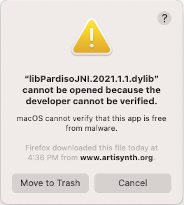
\includegraphics[]{images/MacSecurityNotice}
\else
  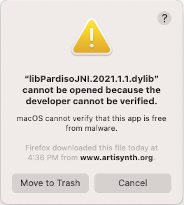
\includegraphics[width=2in]{images/MacSecurityNotice}
\fi
\end{center}
The problem here is that one or more of the native libraries are not ``known''
to Apple and are therefore not trusted. Clicking the "?" on the popup will
open a window containing more information about what to do.

The short version is to immediately open {\sf System Settings > Privacy
\& Security} after the error occurs. Near the bottom, under {\sf
Security}, you should see a notification about the blocked library with
a button to the right labeled {\sf Open Anyway}. Clicking that button
will grant the library a security exception. You will then need to exit
and restart ArtiSynth.

\end{document}
